\documentclass{beamer}
\usetheme{default}
\usepackage{thumbpdf}
\usepackage{wasysym}
\usepackage{ucs}
\usepackage[utf8]{inputenc}
\usepackage{pgf,pgfarrows,pgfnodes,pgfautomata,pgfheaps,pgfshade}
\usepackage{verbatim}
\usepackage{listings}
\usepackage{color}

\definecolor{dkgreen}{rgb}{0,0.6,0}
\definecolor{gray}{rgb}{0.5,0.5,0.5}
\definecolor{mauve}{rgb}{0.58,0,0.82}

\lstset{ %
  backgroundcolor=\color{white},  % choose the background color; you must add \usepackage{color} or \usepackage{xcolor}
  basicstyle=\footnotesize,       % the size of the fonts that are used for the code
  breakatwhitespace=false,        % sets if automatic breaks should only happen at whitespace
  breaklines=true,                % sets automatic line breaking
  captionpos=b,                   % sets the caption-position to bottom
  commentstyle=\color{dkgreen},   % comment style
  deletekeywords={...},           % if you want to delete keywords from the given language
  escapeinside={\%*}{*)},         % if you want to add LaTeX within your code
  extendedchar=true,              % lets you use non-ASCII characters; for 8-bits encodings only, does not work with UTF-8
  frame=single,                   % adds a frame around the code
  keywordstyle=\color{blue},      % keyword style
  language=Octave,                % the language of the code
  morekeywords={*,...},           % if you want to add more keywords to the set
  numbers=left,                   % where to put the line-numbers; possible values are (none, left, right)
  numbersep=5pt,                  % how far the line-numbers are from the code
  numberstyle=\tiny\color{gray},  % the style that is used for the line-numbers
  rulecolor=\color{black},        % if not set, the frame-color may be changed on line-breaks within not-black text (e.g. comments (green here))
  showspaces=false,               % show spaces everywhere adding particular underscores; it overrides 'showstringspaces'
  showstringspaces=false,         % underline spaces within strings only
  showtabs=false,                 % show tabs within strings adding particular underscores
  stepnumber=2,                   % the step between two line-numbers. If it's 1, each line will be numbered
  stringstyle=\color{mauve},      % string literal style
  tabsize=2,                      % sets default tabsize to 2 spaces
  title=\lstname                  % show the filename of files included with \lstinputlisting; also try caption instead of title
}


\lstset{language=C,
  basicstyle=\footnotesize\ttfamily,
  keywordstyle=\footnotesize\color{blue}\ttfamily,
  moredelim=**[is][\btHL]{`}{`},
}

\begin{document}

\pdfinfo
    {
      /Title       (Formation Git)
      /Creator     (Tex)
      /Author      (Nicolas Aguirre)
    }


    \title{Formation GIT}
    \subtitle{Git FTW!}
    \author{Nicolas Aguirre}
    \date{11 Mars 2013}

    \frame{\titlepage}

    \section{Introduction}
    \begin{frame}
      \frametitle{Historique}
      \begin{itemize}
      \item Projet initié par Linus Torvalds pour le noyau linux.
      \item Premiére version le 7 Avril 2005.
      \item Logiciel de gestion de versions decentralisé.
      \item Semblable à Mercurial ou Bitkeeper
      \item Version actuelle 1.8.0
      \item Licence GPLv2
      \item http://git-scm.com
      \end{itemize}
    \end{frame}
%-------------------------------------------------------------------------------
    \section{Workflows}
    \begin{frame}
      \frametitle{Workflows}
      \begin{itemize}
        \item GIT != SVN
        \item Ne jamais se demander quelle est la version SVN de cette commande
        \item svn add != git add
        \item Dans svn trunk est LA branche
        \item Dans git master est UNE branche parmis d'autres
      \end{itemize}
    \end{frame}
    
    \begin{frame}
      \frametitle{Workflow développeur}
      \begin{itemize}
        \item creer une branche de dev
        \item Commiter comme bon vous semble
        \item Aussi souvent que vous voulez
        \item Quand vous voulez
        \item Pusher ou merger les commits en ensembles cohérents
      \end{itemize}
    \end{frame}

    \begin{frame}
      \frametitle{Workflow développeur}
      \begin{itemize}
        \item Supprime la peur de ne pas être à jour.
        \item Permet de faire de la revue de code sur des ensembles cohérents.
        \item Permet de travailler par fonctionnalités.
        \item Permet d'expérimenter dans des branches.
        \item Le développeur deviens un producteur de code source.
      \end{itemize}
    \end{frame}

    \begin{frame}
      \frametitle{Workflow de l'intégrateur}
      \begin{itemize}
        \item Récupération des commits dans une branche
        \item Intégration par fonctionalités
        \item Test des fonctionalités
      \end{itemize}
    \end{frame}
%-------------------------------------------------------------------------------
    \section{Les informations de commits}

    \begin{frame}
      \frametitle{Comment sont stockées les données dans SVN}
      \begin{itemize}
        \item Dans SVN l'information d'un commit est stockée sous forme de différences :
         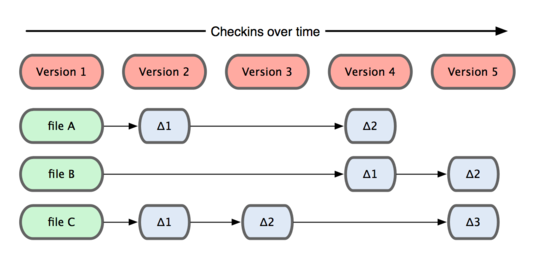
\includegraphics[width=8cm]{imgs/deltas.eps}
      \end{itemize}
    \end{frame}

   \begin{frame}
      \frametitle{Comment sont stockées les données dans GIT}
      \begin{itemize}
        \item Git fait un snapshot des fichiers a chaque version:
         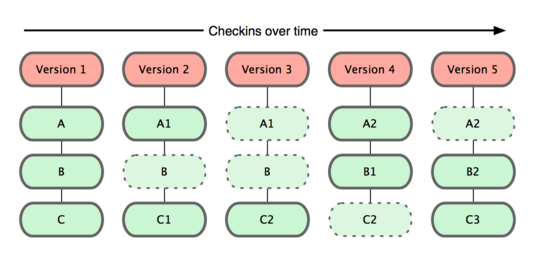
\includegraphics[width=8cm]{imgs/snapshot.eps}
      \end{itemize}
    \end{frame}

   \begin{frame}
      \frametitle{Toutes les informations sont stockées en local}
      \begin{itemize}
        \item toutes les informations sont stockées en local sur votre disque
        \item pas de latence due au réseau
        \item l'historique de tout le projet est local par exemple
        \item Toutes les objets git sont Hashés en SHA-1
      \end{itemize}
    \end{frame}
%-------------------------------------------------------------------------------
   \section{les 3 zones}

   \begin{frame}
     \frametitle{Les 3 zones}
     \begin{itemize}
     \item \alert{La chose la plus importante a retenir !}
     \item la zone ``working directory''
     \item la zone ``staging area''
     \item la zone ``git directory(repository)''
     \item \alert{La chose la plus importante a retenir !}
     \end{itemize}
   \end{frame}

  \begin{frame}
     \frametitle{Les 3 zones}
     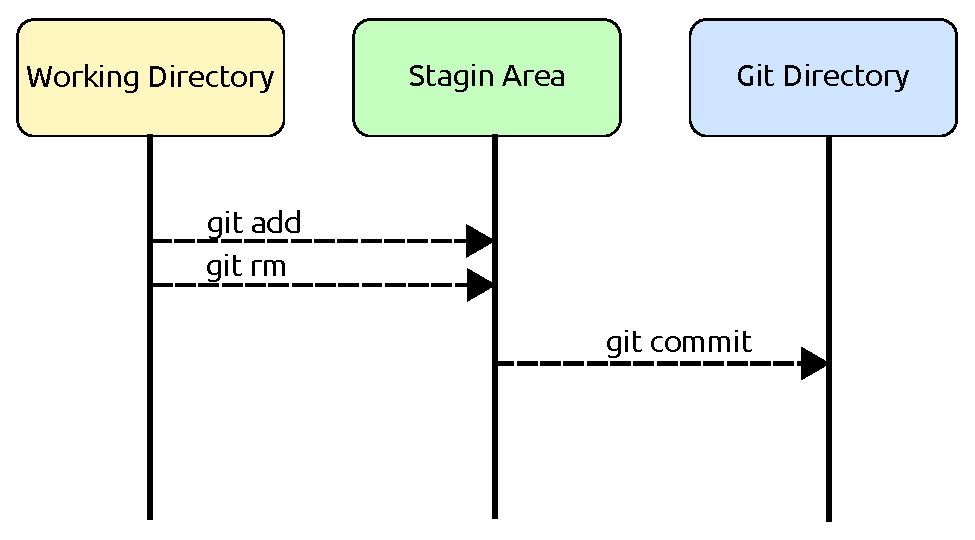
\includegraphics[width=11cm]{imgs/3zones.eps}
  \end{frame}

  \begin{frame}
     \frametitle{Git directory}
     \begin{itemize}
     \item C'est ce qui est copié lorsque vous clonez un repository d'un autre endroit.
     \item C'est la base de donnée de git, c'est l'endroit où il stocke tous les commits, et toutes les relations entre commits.
     \end{itemize}
   \end{frame}

  \begin{frame}
     \frametitle{Working directory}
     \begin{itemize}
     \item C'est un snapshot d'une des version du projet.
     \item Les fichiers sont issues de la base de donnée du git directory.
     \item git les placent sur le disque pour que vous puissiez les utiliser ou les modifier.
     \end{itemize}
   \end{frame}

  \begin{frame}
     \frametitle{Staging Area}
     \begin{itemize}
     \item C'est un fichier qui contient les informations de ce qui ira dans votre prochain commit.
     \item Les fichiers sont issues de la base de donnée du git directory.
     \item git les placent sur le disque pour que vous puissiez les utiliser ou les modifier.
     \end{itemize}
   \end{frame}

  \begin{frame}
     \frametitle{Mon premier commit}
     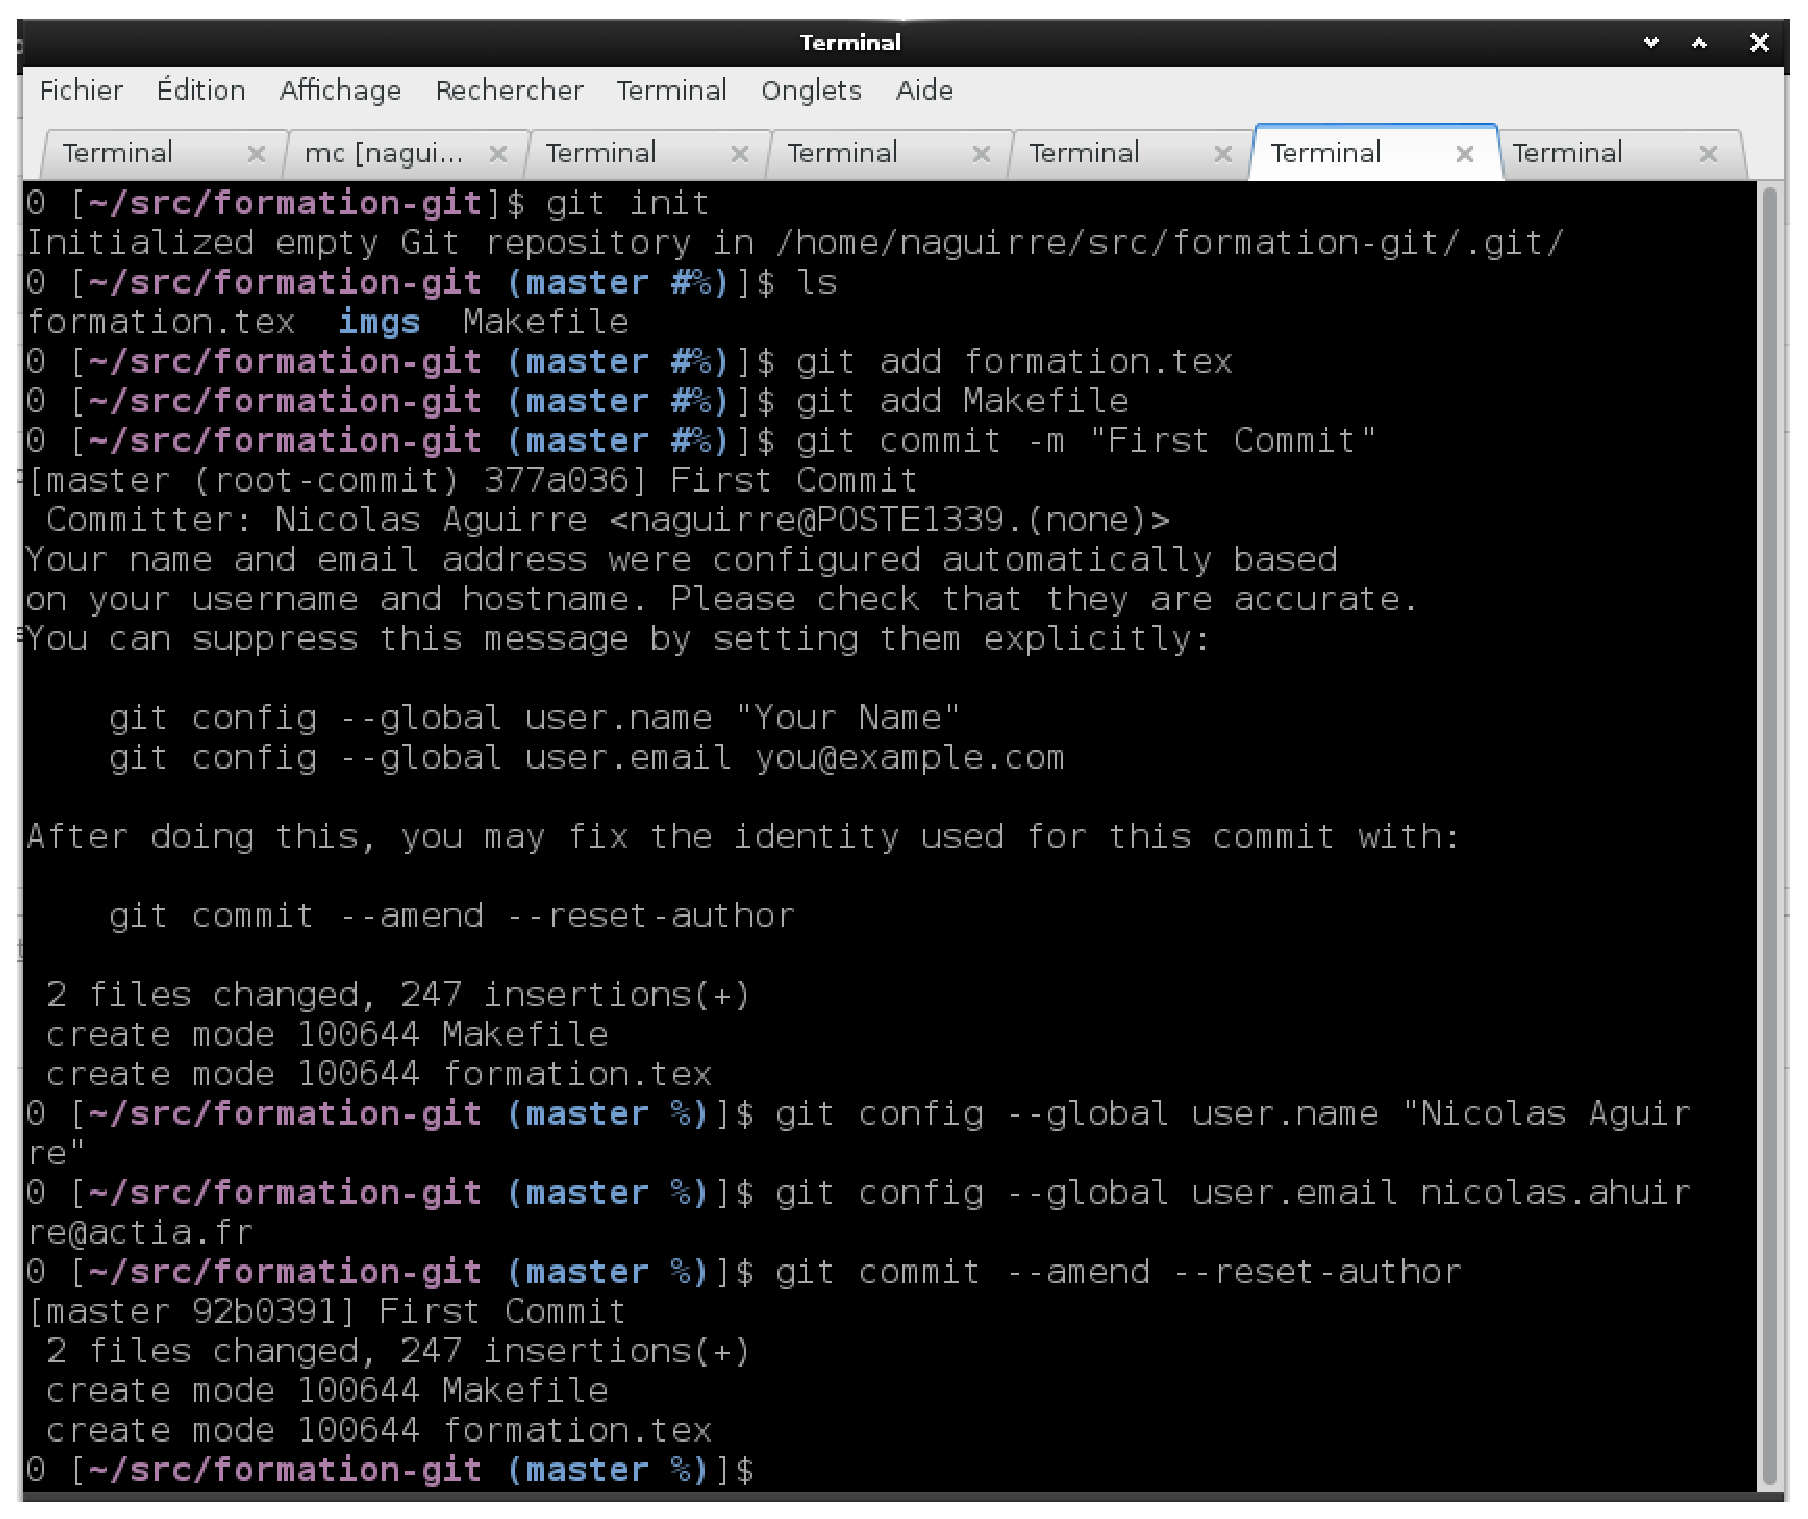
\includegraphics[width=9cm]{imgs/first_commit.eps}
  \end{frame}

  \begin{frame}
     \frametitle{git status}
     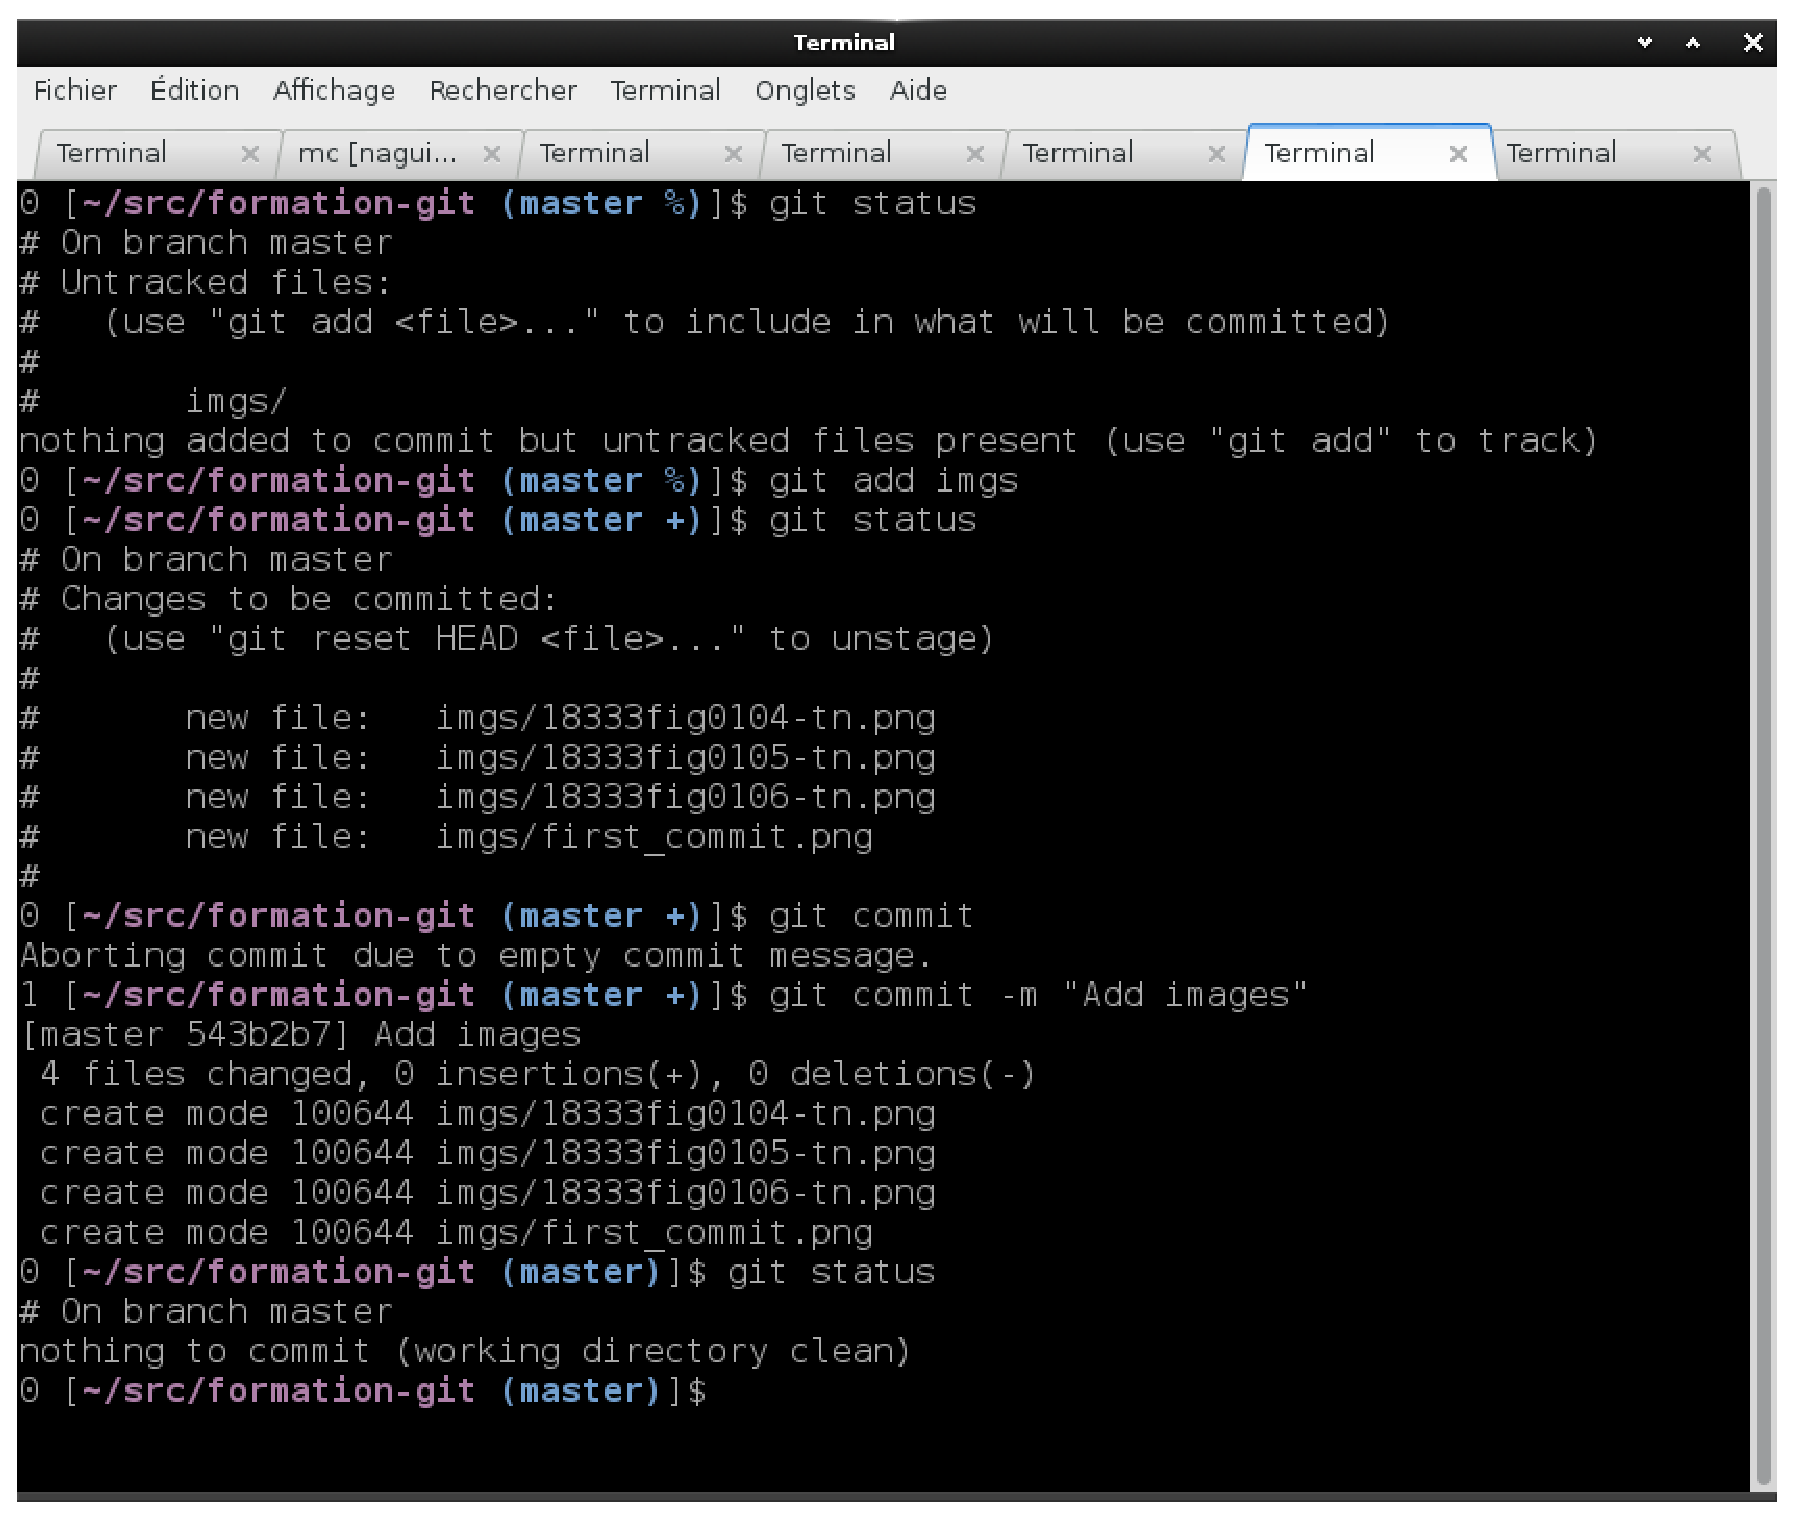
\includegraphics[width=9cm]{imgs/status.eps}
  \end{frame}

\begin{frame}[fragile]\frametitle{Visualisation}
  Historique des commits: \verb|git log|

  \begin{semiverbatim}
  \$ \alert{git log}
  \end{semiverbatim}

  Visualisation des différences: \verb|git diff et git diff --staged|
  \begin{semiverbatim}
  \$ \alert{git diff}
  \$ \alert{git diff --staged}
  \end{semiverbatim}

\end{frame}

\begin{frame}[fragile]
  \frametitle{Récapitulatif des commandes}
  \begin{semiverbatim}
    \$ git add
    \$ git commit
    \$ git status
    \$ git diff
    \$ git log
  \end{semiverbatim}


\end{frame}

%-------------------------------------------------------------------------------

\section{Travailler avec des serveurs distants}
\begin{frame}
  \frametitle{Buildroot}
  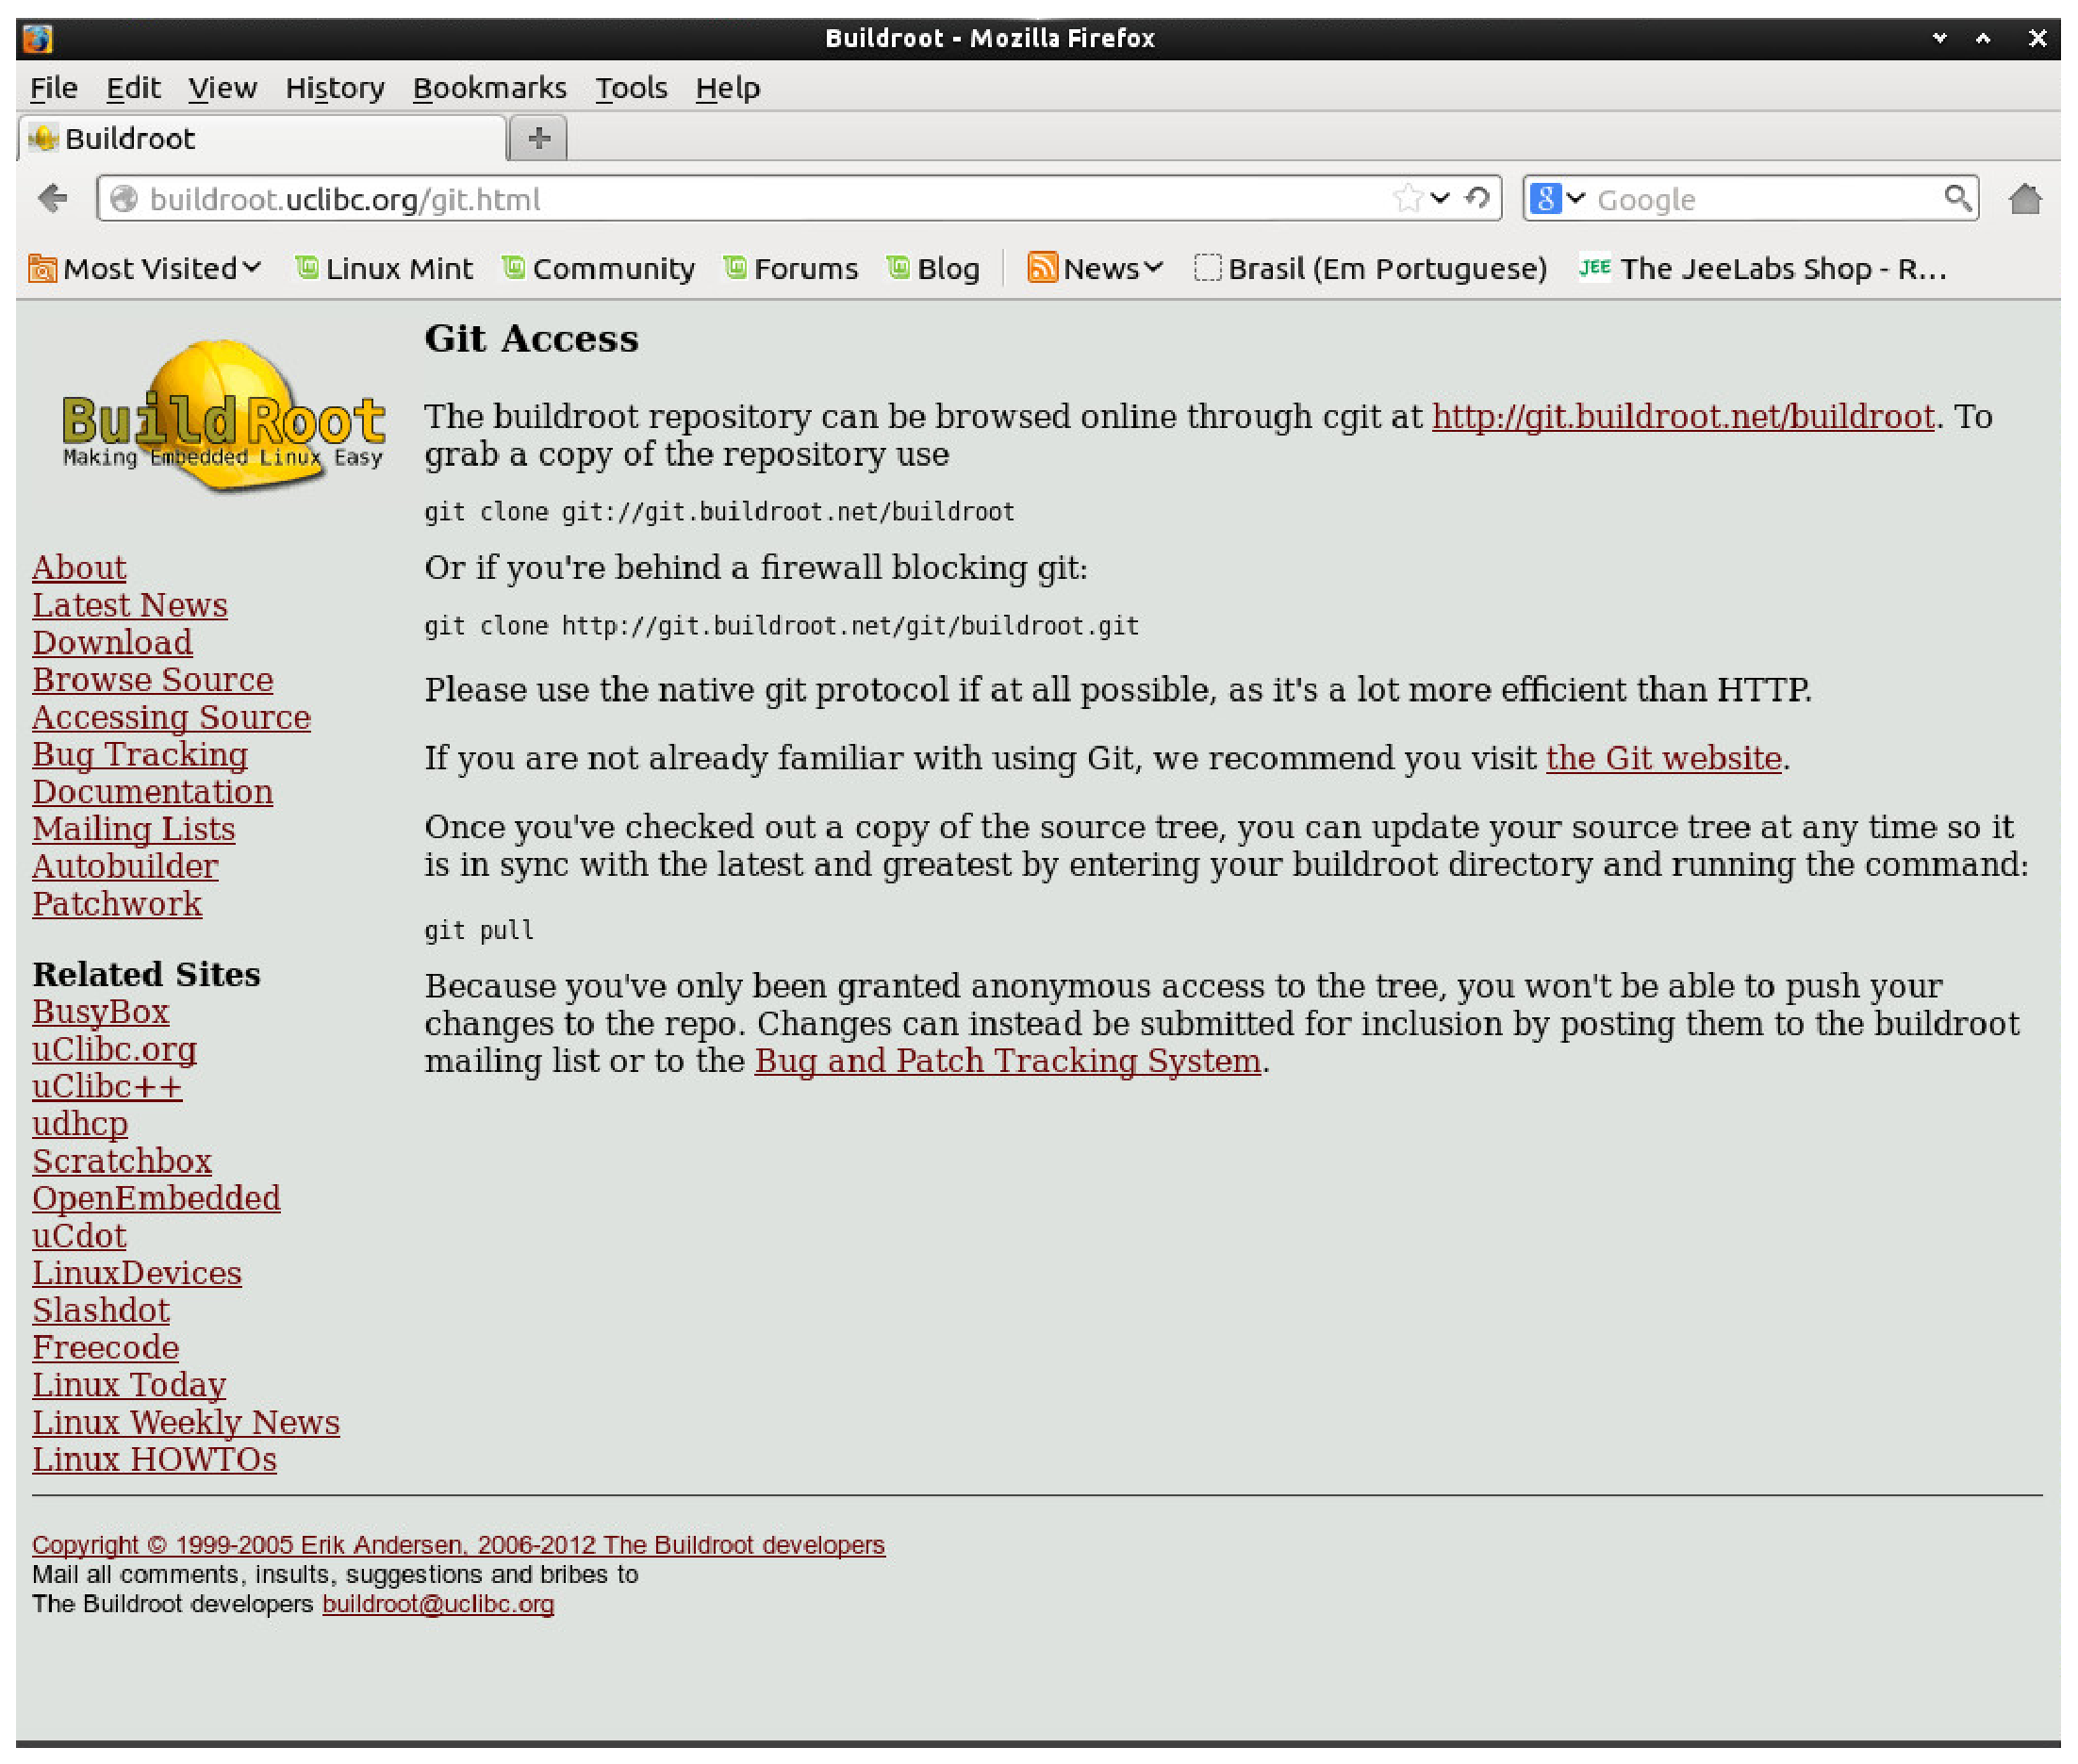
\includegraphics[width=9cm]{imgs/buildroot.eps}
\end{frame}


\begin{frame}
  \frametitle{git clone}
  \begin{semiverbatim}
    \$ git clone http://git.buildroot.net/git/buildroot.git
  \end{semiverbatim}
\end {frame}


\begin{frame}
  \frametitle{Outil graphique: git}
  \begin{itemize}
  \item gitg est un outil graphique permettant de visualiser plus facilement l'arbre de commits.
  \item il existe egalement tig ou tortoise git sur windows
  \end{itemize}
\end{frame}

\begin{frame}
  \frametitle{Seveurs distants}
  \begin{semiverbatim}
    \$ git remote -v

    origin git://git.buildroot.net/buildroot (fetch)

    origin git://git.buildroot.net/buildroot (push)
  \end{semiverbatim}
\end{frame}

\begin{frame}
  \frametitle{Récapitulatif des commandes}
  \begin{itemize}
  \item push : action d'envoyer les commits ainsi que les relations entre commits vers le serveur distant (origin par défaut)
  \item fetch : action de récuéprer les commits ainsi que les relations entre commits depuis le serveur distant
  \end{itemize}
\end{frame}

\begin{frame}
  \frametitle{Ajout d'un serveur}
  \begin{semiverbatim}
    \$ git remote add forge3 git@forge3:buildroot

    \$ git remote -v

    origin git@forge3:buildroot (fetch)

    origin git@forge3:buildroot (push)

  \end{semiverbatim}
\end{frame}

\begin{frame}
  \frametitle{Checkout}
  \begin{semiverbatim}
    \$ git checkout tag/sha1/branch
    
    Git présente dans le systeme de fichier la version qu'on lui demande.
  \end{semiverbatim}
\end{frame}

\end{document}
